% --
% wavenets

\section{Experiments on Wavenets}\label{exp_wavenet}
\thesisStateReady
Very few experiments were performed on the Wavenet architecture shown in \rsec{nn_arch_wavenet}, because of its complex model structure and heavy computational footprint.
It took much training time and energy consumption for few epochs, further the results on the accuracy of classifying speech commands were really bad.
This architecture is therefore left for future research.
Nevertheless the best performing model was trained with 500 examples per label of the L12 labels, 100 epochs, a learning rate of $0.001$ for 10 epochs and the changing to $0.0001$ and a usual batch size of 32.
The accuracy score for the training and the confusion matrix is shown in \rfig{exp_wavenet_acc} and \rfig{exp_wavenet_confusion}.
\begin{figure}[!ht]
  \centering
  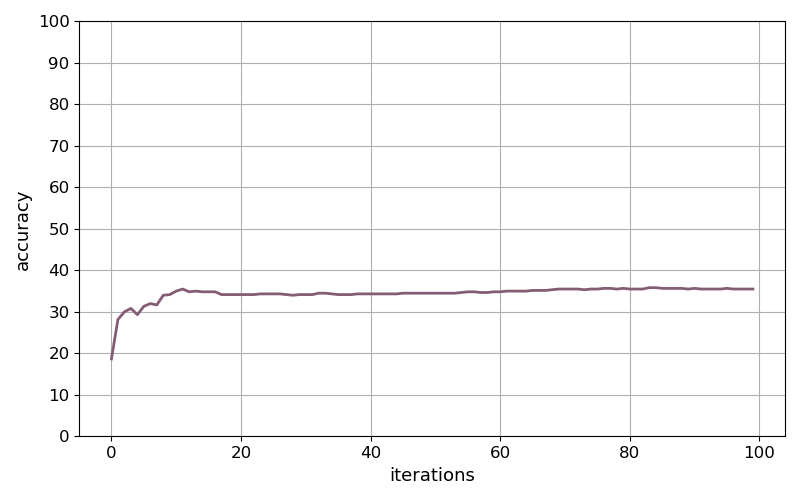
\includegraphics[width=0.45\textwidth]{./5_exp/figs/exp_wavenet_acc}
  \caption{Accuracies on the validation set during the training of the Wavenet model with classification extension.}
  \label{fig:exp_wavenet_acc}
\end{figure}
\FloatBarrier
\noindent
\begin{figure}[!ht]
  \centering
  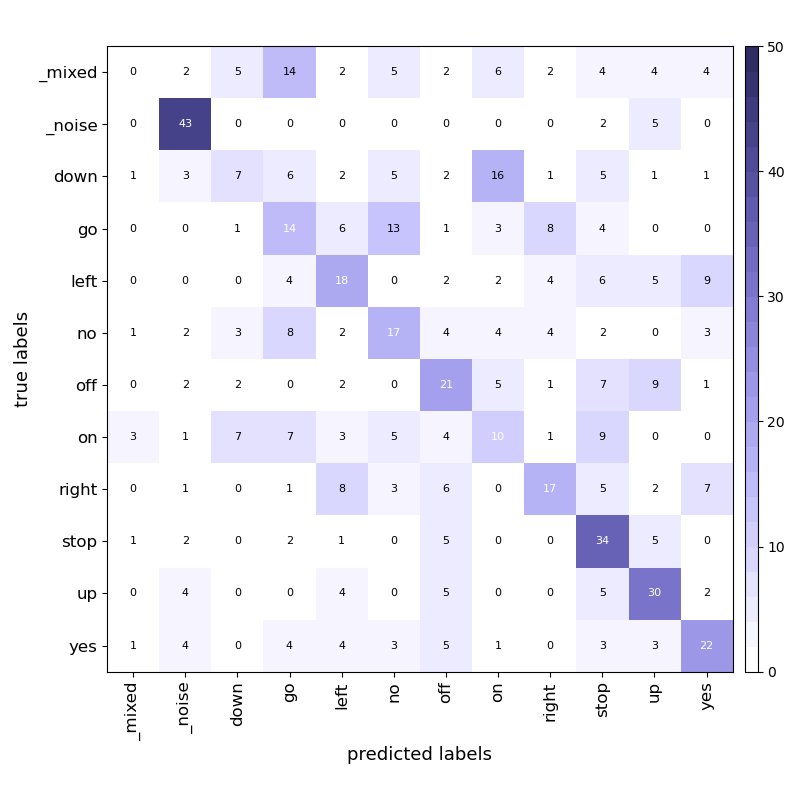
\includegraphics[width=0.45\textwidth]{./5_exp/figs/exp_wavenet_confusion_test}
  \caption{Confusion matrix of the test set evaluated on the trained Wavenet model.}
  \label{fig:exp_wavenet_confusion}
\end{figure}
\FloatBarrier
\noindent
The best test accuracy was \SI{38.83}{\percent}, a confusion matrix is shown in \rfig{exp_wavenet_confusion}.

% \begin{figure}[!ht]
%   \centering
%   \subfigure[Accuracy]{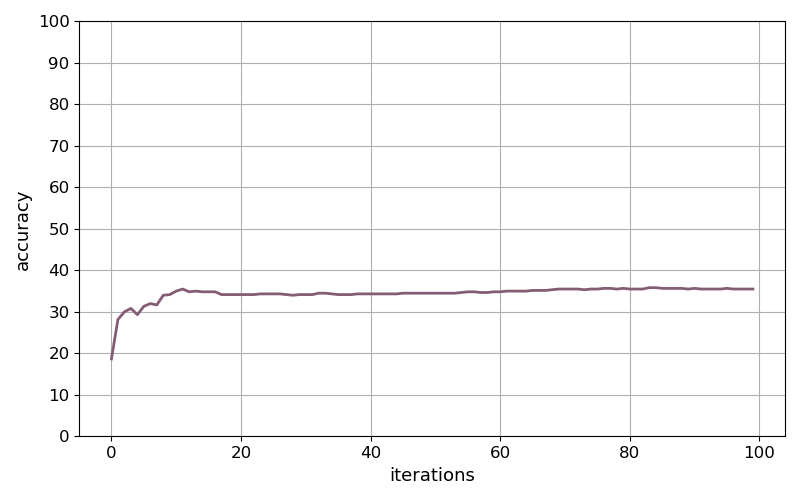
\includegraphics[height=0.4\textwidth]{./5_exp/figs/exp_wavenet_acc}}
%   \subfigure[Confusion matrix]{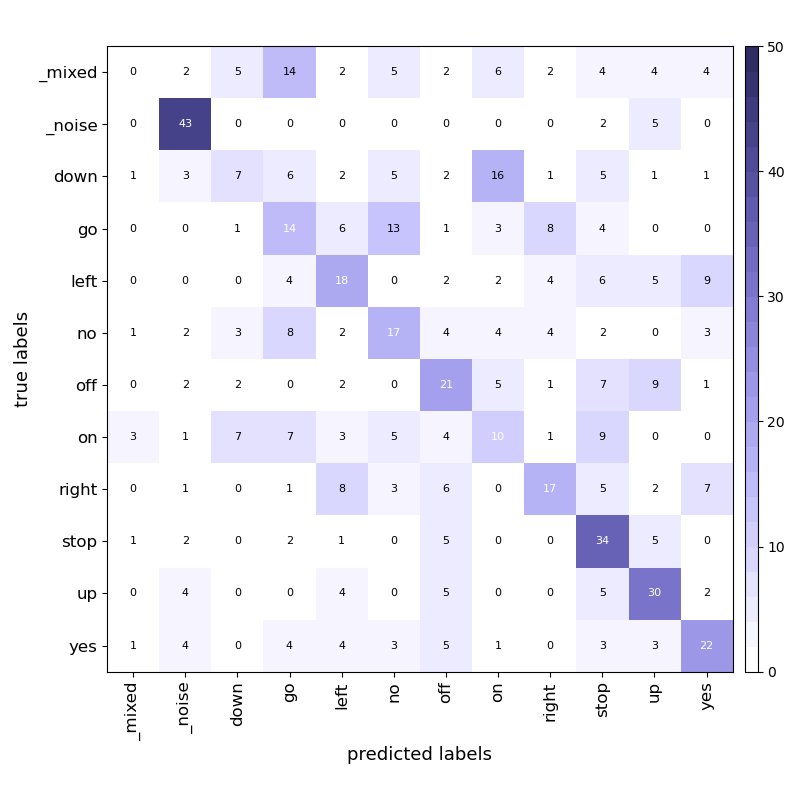
\includegraphics[height=0.4\textwidth]{./5_exp/figs/exp_wavenet_confusion_test}}
%   \caption{Accuracy on the validation set and confusion matrix on the test set of the trained Wavenet model.}
%   \label{fig:exp_wavenet}
% \end{figure}
% \FloatBarrier
% \noindent